% Created 2022-07-21 Thu 13:39
% Intended LaTeX compiler: pdflatex
\documentclass[11pt]{article}
\usepackage[utf8]{inputenc}
\usepackage[T1]{fontenc}
\usepackage{graphicx}
\usepackage{longtable}
\usepackage{wrapfig}
\usepackage{rotating}
\usepackage[normalem]{ulem}
\usepackage{amsmath}
\usepackage{amssymb}
\usepackage{capt-of}
\usepackage{hyperref}
\author{Josh Kwok}
\date{\today}
\title{}
\hypersetup{
 pdfauthor={Josh Kwok},
 pdftitle={},
 pdfkeywords={},
 pdfsubject={},
 pdfcreator={Emacs 29.0.50 (Org mode 9.5.1)},
 pdflang={English}}
\begin{document}

\tableofcontents \clearpage\section{Week 2}
\label{week-2}
\section{Week2 Assignments}
\label{week2-assignments}
\subsection{Assignment Selection}
\label{assignment-selection}
We offer 3 assignments, so you can choose one or more depending on your situation.

\href{https://www.notion.so/dc0c5f6e11c441779bed71ec77cd7118}{Untitled}

\begin{quote}
Bonus points for completing multiple assignments !!!
\end{quote}

\subsection{Assignment 1. Polynomial Solving and Proving}
\label{assignment-1.-polynomial-solving-and-proving}
Define the following function with 3 variables \(a, b, c\).

\begin{verbatim}
def f(a, b, c):
  if a == 1:
    return b*c
  return 2b - c
}
\end{verbatim}

Polynomial solving and polynomial proving are very important parts of zkSNARKs, while Groth16 and Plonk representations of circuit constraints differently, completing the following polynomial-related problem solving and deduction.

\begin{quote}
Tips: Refer to Why and How zk-SNARK Works: Definitive Explanation for help.
\end{quote}

\subsubsection{Q1}
\label{q1}
To convert the function to circuit of R1CS form (flatten), use polynomial interpolation with values\((1,2,3,...)\) to solve variable polynomials for each variables (including intermediate variables).

\subsubsection{A1}
\label{a1}
Since \(x\) is only part of the conditional, we can make a strong assumption that \(x \in \{0,1\}\). The function is equivalent to this function:

\(f(x,y,z)=x \cdot y \cdot z + (x-1)\cdot(2 y- z)\)

s.t.

\(x \cdot (x-1) = 0\)

The circuit looks like below:

\begin{figure}[htbp]
\centering
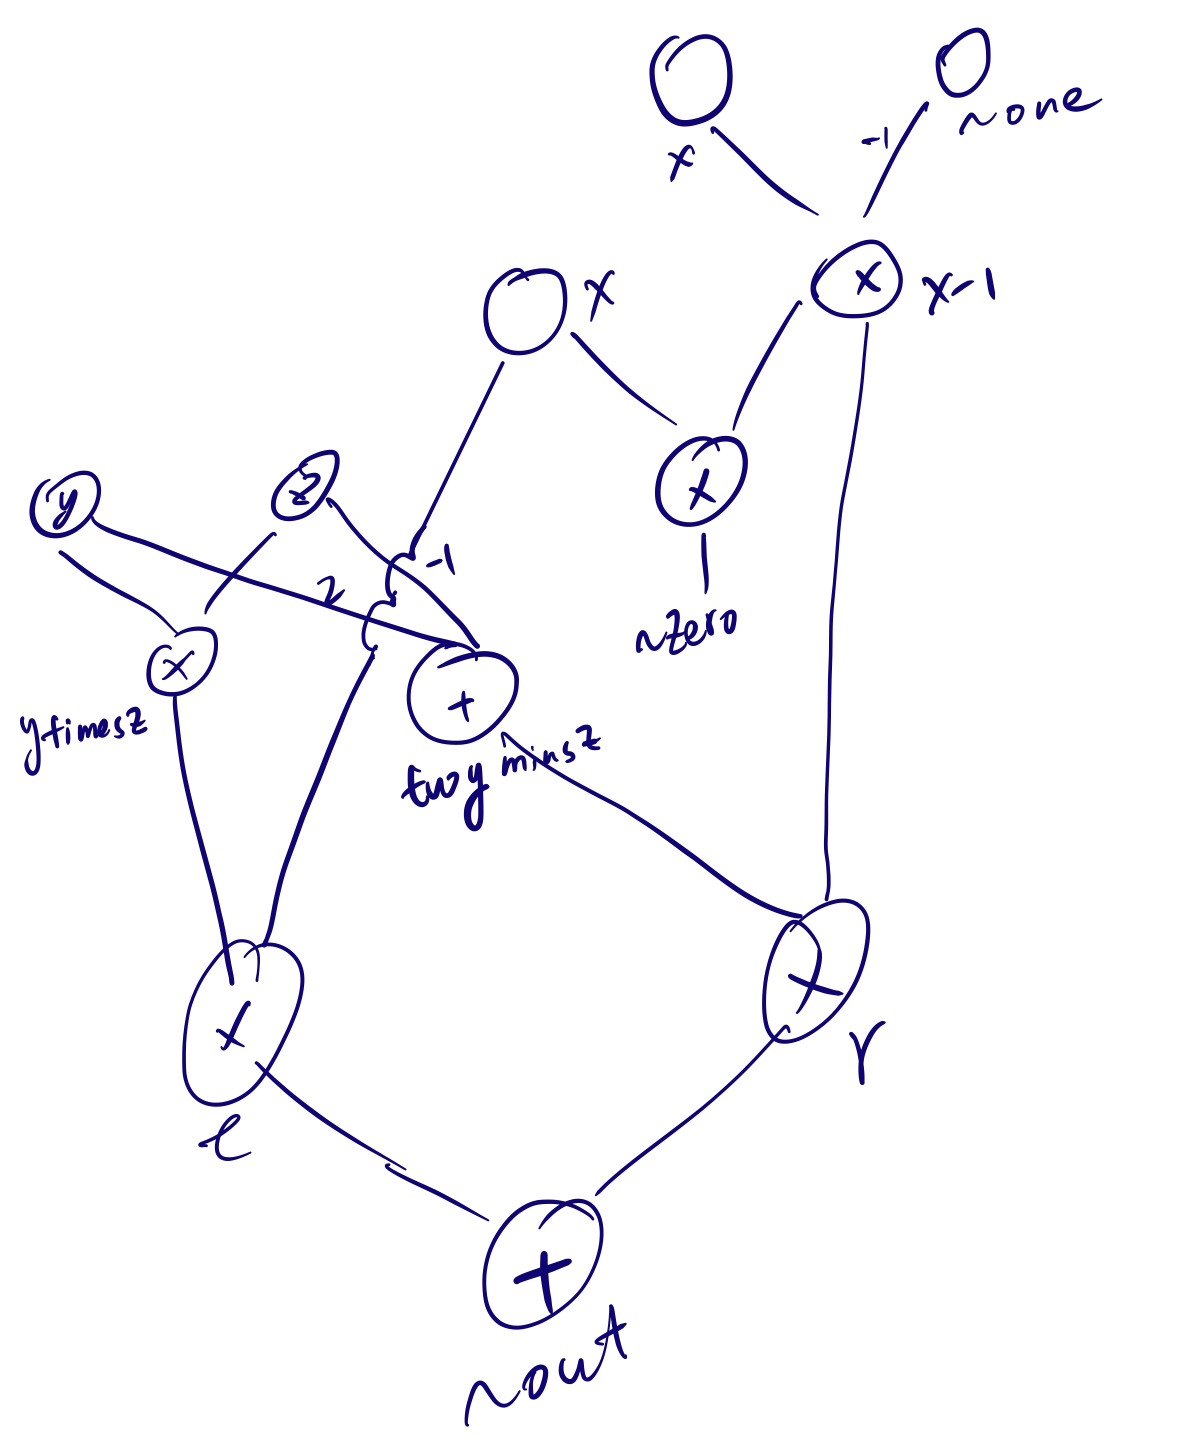
\includegraphics[width=.9\linewidth]{./img/1.png}
\caption{Untitled}
\end{figure}

i.e. for variable mapping:

\(\sim{one},x,y,z,xminu1,ytimesz,twoyminusz,l,r,\sim{out}\)

s.t.

\begin{enumerate}
\item \(xminus1 = x \cdot \sim{one} + (-1) * \sim{one}\)
\item \(x * xminus1=0\)
\item \(ytimesz = y * z\)
\item \(twoyminusz = 2 \cdot \sim{one} \cdot y - z\)
\item \(l = ytimesz * x\)
\item \(r = twoyminusz * xminus1\)
\item \(\sim{out} = l + r\)
\end{enumerate}

For each numbered gate:

\begin{enumerate}
\item
\end{enumerate}

\(a = [0,1,0,0,0,0,0,0,0,0]\)

\(b=[1,0,0,0,0,0,0,0,0,0]\)

\(c=[1,0,0,0,1,0,0,0,0,0]\)

\begin{enumerate}
\item
\end{enumerate}

\(a = [0,1,0,0,0,0,0,0,0,0]\)

\(b=[0,0,0,0,1,0,0,0,0,0]\)

\(c=[0,0,0,0,0,0,0,0,0,0]\)

\begin{enumerate}
\item
\end{enumerate}

\(a=[0,0,1,0,0,0,0,0,0,0]\)

\(b=[0,0,0,1,0,0,0,0,0,0]\)

\(c=[0,0,0,0,0,1,0,0,0,0]\)

\begin{enumerate}
\item
\end{enumerate}

\(a=[2,0,0,0,0,0,0,0,0,0]\)

\(b=[0,0,1,0,0,0,0,0,0,0]\)

\(c=[0,0,0,1,0,0,1,0,0,0]\)

\begin{enumerate}
\item
\end{enumerate}

\(a=[0,1,0,0,0,0,0,0,0,0]\)

\(b=[0,0,0,0,0,1,0,0,0,0]\)

\(c=[0,0,0,0,0,0,0,1,0,0]\)

\begin{enumerate}
\item
\end{enumerate}

\(a=[0,0,0,0,1,0,0,0,0,0]\)

\(b=[0,0,0,0,0,0,1,0,0,0]\)

\(c=[0,0,0,0,0,0,0,0,1,0]\)

\begin{enumerate}
\item
\end{enumerate}

\(a=[0,0,0,0,0,0,0,1,0,0]\)

\(b=[0,0,0,0,0,0,0,0,1,0]\)

\(c=[0,0,0,0,0,0,0,0,0,1]\)

The complete R1CS put together is:

\(A\)

\(\begin{vmatrix} 0,1,0,0,0,0,0,0,0,0 \\ 0,1,0,0,0,0,0,0,0,0 \\ 0,0,1,0,0,0,0,0,0,0 \\ 2,0,0,0,0,0,0,0,0,0 \\ 0,1,0,0,0,0,0,0,0,0 \\ 0,0,0,0,1,0,0,0,0,0 \\ 0,0,0,0,0,0,0,1,0,0 \\ \end{vmatrix}\)

B

\(\begin{vmatrix} 1,0,0,0,0,0,0,0,0,0 \\ 0,0,0,0,1,0,0,0,0,0 \\ 0,0,0,1,0,0,0,0,0,0 \\ 0,0,1,0,0,0,0,0,0,0 \\ 0,0,0,0,0,1,0,0,0,0 \\ 0,0,0,0,0,0,1,0,0,0 \\ 0,0,0,0,0,0,0,0,1,0 \\ \end{vmatrix}\)

C

\(\begin{vmatrix} 1,0,0,0,1,0,0,0,0,0 \\ 0,0,0,0,0,0,0,0,0,0 \\ 0,0,0,0,0,1,0,0,0,0 \\ 0,0,0,1,0,0,1,0,0,0 \\ 0,0,0,0,0,0,0,1,0,0 \\ 0,0,0,0,0,0,0,0,1,0 \\ 0,0,0,0,0,0,0,0,0,1 \\ \end{vmatrix}\)

Use Lanrange interpolation to get the variable polynomials for:

\begin{verbatim}
:'
For A:
x    1,2,3,4,5,6,7
  +-----------------
1 |[[0,0,0,2,0,0,0],
2 | [1,1,0,0,1,0,0],
3 | [0,0,1,0,0,0,0],
4 | [0,0,0,0,0,0,0],
5 | [0,0,0,0,0,1,0],
6 | [0,0,0,0,0,0,0],
7 | [0,0,0,0,0,0,0],
8 | [0,0,0,0,0,0,1],
9 | [0,0,0,0,0,0,0],
10| [0,0,0,0,0,0,0]]

For B:
x    1,2,3,4,5,6,7
  +-----------------
1 |[[1,0,0,0,0,0,0],
2 | [0,0,0,0,0,0,0],
3 | [0,0,0,1,0,0,0],
4 | [0,0,1,0,0,0,0],
5 | [0,1,0,0,0,0,0],
6 | [0,0,0,0,1,0,0],
7 | [0,0,0,0,0,1,0],
8 | [0,0,0,0,0,0,0],
9 | [0,0,0,0,0,0,1],
10| [0,0,0,0,0,0,0]]

For C:
x    1,2,3,4,5,6,7
  +----------------
1 |[[1,0,0,0,0,0,0],
2 | [0,0,0,0,0,0,0],
3 | [0,0,0,0,0,0,0],
4 | [0,0,0,1,0,0,0],
5 | [1,0,0,0,0,0,0],
6 | [0,0,1,0,0,0,0],
7 | [0,0,0,1,0,0,0],
8 | [0,0,0,0,1,0,0],
9 | [0,0,0,0,0,1,0],
10| [0,0,0,0,0,0,1]]
'
\end{verbatim}

Use the following Python code to compute:

\begin{verbatim}
from scipy.interpolate import lagrange
import numpy as np
from numpy.polynomial import polynomial as P

np.set_printoptions(precision=2)

def poly_interpolate(index, matrics):
    res = []
    for row in matrics:
        poly = lagrange(index, row).coef[::-1]
        res.append(poly)
    return np.array(res, dtype=object)

def polymuln(lst):
    if len(lst) == 0:
        return 1
    return P.polymul(lst[0], polymuln(lst[1:]))

def QAP(s, A, B, C):
    L = np.matmul(s, A)
    R = np.matmul(s, B)
    O = np.matmul(s, C)
    print(f"L: {L}")
    print(f"R: {R}")
    print(f"O: {O}")
    Q = P.polysub(P.polymul(L, R), O)
    print(f"T:\n {Q}")
    assert len(L) == len(R) == len(O)
    return P.polydiv(Q, Z(len(L)))

def Z(n):
    ns = [[-(1 + i), 1] for i, _ in enumerate(range(n))]
    return polymuln(ns)

def main(s, A, B, C):
    x = np.arange(1, len(A) + 1)

    resA = poly_interpolate(x, np.transpose(A))
    resB = poly_interpolate(x, np.transpose(B))
    resC = poly_interpolate(x, np.transpose(C))

    print(f"resA: \n {resA}")
    print(f"resB: \n {resB}")
    print(f"resC: \n {resC}")

    return QAP(s, resA, resB, resC)

# variables: \sim{one},x,y,z,xminu1,ytimesz,twoyminusz,l,r,\sim{out}
s = np.array([1, 0, 11, 5, 0, 55, 17, 0, -17, -17])

A = np.array(
    [
        [0, 1, 0, 0, 0, 0, 0, 0, 0, 0],
        [0, 1, 0, 0, 0, 0, 0, 0, 0, 0],
        [0, 0, 1, 0, 0, 0, 0, 0, 0, 0],
        [2, 0, 0, 0, 0, 0, 0, 0, 0, 0],
        [0, 1, 0, 0, 0, 0, 0, 0, 0, 0],
        [0, 0, 0, 0, 1, 0, 0, 0, 0, 0],
        [0, 0, 0, 0, 0, 0, 0, 1, 0, 0],
    ]
)

B = np.array(
    [
        [1, 0, 0, 0, 0, 0, 0, 0, 0, 0],
        [0, 0, 0, 0, 1, 0, 0, 0, 0, 0],
        [0, 0, 0, 1, 0, 0, 0, 0, 0, 0],
        [0, 0, 1, 0, 0, 0, 0, 0, 0, 0],
        [0, 0, 0, 0, 0, 1, 0, 0, 0, 0],
        [0, 0, 0, 0, 0, 0, 1, 0, 0, 0],
        [0, 0, 0, 0, 0, 0, 0, 0, 1, 0],
    ]
)

C = np.array(
    [
        [1, 0, 0, 0, 1, 0, 0, 0, 0, 0],
        [0, 0, 0, 0, 0, 0, 0, 0, 0, 0],
        [0, 0, 0, 0, 0, 1, 0, 0, 0, 0],
        [0, 0, 0, 1, 0, 0, 1, 0, 0, 0],
        [0, 0, 0, 0, 0, 0, 0, 1, 0, 0],
        [0, 0, 0, 0, 0, 0, 0, 0, 1, 0],
        [0, 0, 0, 0, 0, 0, 0, 0, 0, 1],
    ]
)

# print(main(s, A, B, C))

# A = np.array(
#     [
#         [0, 1, 0, 0, 0, 0],
#         [0, 0, 0, 1, 0, 0],
#         [0, 1, 0, 0, 1, 0],
#         [5, 0, 0, 0, 0, 1],
#     ]
# )

# B = np.array(
#     [
#         [0, 1, 0, 0, 0, 0],
#         [0, 1, 0, 0, 0, 0],
#         [1, 0, 0, 0, 0, 0],
#         [1, 0, 0, 0, 0, 0],
#     ]
# )

# C = np.array(
#     [
#         [0, 0, 0, 1, 0, 0],
#         [0, 0, 0, 0, 1, 0],
#         [0, 0, 0, 0, 0, 1],
#         [0, 0, 1, 0, 0, 0],
#     ]
# )

# A_ = np.array(
#     [
#         [-5.0, 9.166, -5.0, 0.833],
#         [8.0, -11.333, 5.0, -0.666],
#         [0.0, 0.0, 0.0, 0.0],
#         [-6.0, 9.5, -4.0, 0.5],
#         [4.0, -7.0, 3.5, -0.5],
#         [-1.0, 1.833, -1.0, 0.166],
#     ]
# )
# B_ = np.array(
#     [
#         [3.0, -5.166, 2.5, -0.333],
#         [-2.0, 5.166, -2.5, 0.333],
#         [0.0, 0.0, 0.0, 0.0],
#         [0.0, 0.0, 0.0, 0.0],
#         [0.0, 0.0, 0.0, 0.0],
#         [0.0, 0.0, 0.0, 0.0],
#     ]
# )
# C_ = [
#     [0.0, 0.0, 0.0, 0.0],
#     [0.0, 0.0, 0.0, 0.0],
#     [-1.0, 1.833, -1.0, 0.166],
#     [4.0, -4.333, 1.5, -0.166],
#     [-6.0, 9.5, -4.0, 0.5],
#     [4.0, -7.0, 3.5, -0.5],
# ]
# s = np.array([1, 3, 35, 9, 27, 30])

# print(main(s, A, B, C))
\end{verbatim}

For variables \(\sim{one} (1),x (2),y (3),z (4),xminu1 (5),ytimesz (6),twoyminusz (7),l (8),r (9),\sim{out} (10)\) in R1CS flatten format:

\(A\) variable polynomials with coefficients:

\(\begin{pmatrix} \sim{one} \\ x \\ y \\ z \\ xminu1 \\ ytimesz \\ twoyminusz \\ l \\ r \\ \sim{out} \\ \end{pmatrix} = \begin{pmatrix} -7.00e+01& 1.64e+02& -1.41e+02& 5.87e+01& -1.26e+01& 1.33e+00& -5.56e-02 \\ 7.00e+00& -1.74e+01& 1.90e+01& -9.75e+00& 2.47e+00& -3.00e-01& 1.39e-02 \\ 3.50e+01& -7.91e+01& 6.48e+01& -2.54e+01& 5.15e+00& -5.21e-01& 2.08e-02 \\ 0&0&0&0&0&0&0 \\ -7.00e+00& 1.70e+01& -1.54e+01& 6.83e+00& -1.58e+00& 1.83e-01& -8.33e-03 \\ 0&0&0&0&0&0&0 \\ 0&0&0&0&0&0&0 \\ 1.00e+00& -2.45e+00& 2.26e+00& -1.02e+00& 2.43e-01& -2.92e-02& 1.39e-03 \\ 0&0&0&0&0&0&0 \\ 0&0&0&0&0&0&0 \\ \end{pmatrix} \cdot \begin{pmatrix} 1 \\ x \\ x^2 \\ x^3 \\ x^4 \\ x5 \\ x6 \end{pmatrix}\)

\(B\) variable polynomials with coefficients:

\(\begin{pmatrix} \sim{one} \\ x \\ y \\ z \\ xminu1 \\ ytimesz \\ twoyminusz \\ l \\ r \\ \sim{out} \\ \end{pmatrix} = \begin{pmatrix} 7.00e+00& -1.12e+01& 7.09e+00& -2.31e+00& 4.10e-01& -3.75e-02& 1.39e-03 \\0&0&0&0&0&0&0 \\-3.50e+01& 8.20e+01& -7.07e+01& 2.93e+01& -6.28e+00& 6.67e-01& -2.78e-02 \\3.50e+01& -7.91e+01& 6.48e+01& -2.54e+01& 5.15e+00& -5.21e-01& 2.08e-02 \\-2.10e+01& 4.40e+01& -3.27e+01& 1.18e+01& -2.25e+00& 2.17e-01& -8.33e-03 \\2.10e+01& -5.02e+01& 4.47e+01& -1.93e+01& 4.31e+00& -4.79e-01& 2.08e-02 \\-7.00e+00& 1.70e+01& -1.54e+01& 6.83e+00& -1.58e+00& 1.83e-01& -8.33e-03 \\0&0&0&0&0&0&0 \\1.00e+00& -2.45e+00& 2.26e+00& -1.02e+00& 2.43e-01& -2.92e-02& 1.39e-03 \\0&0&0&0&0&0&0 \\ \end{pmatrix} \cdot \begin{pmatrix} 1 \\ x \\ x^2 \\ x^3 \\ x^4 \\ x5 \\ x6 \end{pmatrix}\)

\(C\) variable polynomials with coefficients:

\(\begin{pmatrix} \sim{one} \\ x \\ y \\ z \\ xminu1 \\ ytimesz \\ twoyminusz \\ l \\ r \\ \sim{out} \\ \end{pmatrix} = \begin{pmatrix} 7.00e+00& -1.12e+01& 7.09e+00& -2.31e+00& 4.10e-01& -3.75e-02& 1.39e-03 \\ 0&0&0&0&0&0&0 \\ 0&0&0&0&0&0&0 \\ -3.50e+01& 8.20e+01& -7.07e+01& 2.93e+01& -6.28e+00& 6.67e-01& -2.78e-02 \\ 7.00e+00& -1.12e+01& 7.09e+00& -2.31e+00& 4.10e-01& -3.75e-02& 1.39e-03 \\ 3.50e+01& -7.91e+01& 6.48e+01& -2.54e+01& 5.15e+00& -5.21e-01& 2.08e-02 \\ -3.50e+01& 8.20e+01& -7.07e+01& 2.93e+01& -6.28e+00& 6.67e-01& -2.78e-02 \\ 2.10e+01& -5.02e+01& 4.47e+01& -1.93e+01& 4.31e+00& -4.79e-01& 2.08e-02 \\ -7.00e+00& 1.70e+01& -1.54e+01& 6.83e+00& -1.58e+00& 1.83e-01& -8.33e-03 \\ 1.00e+00& -2.45e+00& 2.26e+00& -1.02e+00& 2.43e-01& -2.92e-02& 1.39e-03 \\ \end{pmatrix} \cdot \begin{pmatrix} 1 \\ x \\ x^2 \\ x^3 \\ x^4 \\ x5 \\ x6 \end{pmatrix}\)

\subsubsection{Q2}
\label{q2}
Continuing with Q1, solve for the left operand polynomial L(X), the right operand polynomial R(X), the output operand polynomial O(X), and the target polynomial T(X) = (x-1)(x-2)(x-3)\ldots{} (interpolation of Q1 solution process), after assigning values to the variables (x=1, y=2, z=5)\ldots{} , verify if \(L(X)*R(X) - O(X)\) is divisible by T(X) and why?

\begin{quote}
Note: The polynomial solution problems involved in Q1, Q2 are the very core of Groth16, Pinocchio
\end{quote}

\subsubsection{A2}
\label{a2}
Run the above Python code and the logs returned polynomials with coefficients:

\begin{verbatim}
L: [ 3.15e+02 -7.06e+02  5.72e+02 -2.21e+02  4.40e+01 -4.40e+00  1.74e-01]
R: [ 8.16e+02 -1.94e+03  1.71e+03 -7.33e+02  1.63e+02 -1.80e+01  7.81e-01]
O: [ 1.26e+03 -2.80e+03  2.24e+03 -8.53e+02  1.68e+02 -1.66e+01  6.54e-01]
T: [-5.04e+03  1.31e+04 -1.31e+04  6.77e+03 -1.96e+03  3.22e+02 -2.80e+01
  1.00e+00]
\end{verbatim}

\(L*R-O\) should be divisible by T with zero (almost due to floating point). The reason is:

\begin{quote}


\begin{enumerate}
\item is defined as \texttt{(x - 1) * (x - 2) * (x - 3) ...}  - the simplest polynomial that is equal to zero at all points that correspond to logic gates. It is an elementary fact of algebra that \emph{any}  polynomial that is equal to zero at all of these points has to be a multiple of this minimal polynomial, and if a polynomial is a multiple of Z then its evaluation at any of those points will be zero
\end{enumerate}
\end{quote}

Since \(1,2,\dots,10\) are \(x\) values used in Lagrange interpolation, the curve \(L*R-T\) should have them as roots. As quoted above, all polynomials should be divisible by the product of roots.

\subsubsection{Q3}
\label{q3}
Convert the function into a system of circuit constrained equations (addition, multiplication, input, output, etc.), then convert these circuit constraints into a system of circuit constrained equations of the form defined by Plonk as "(qL) - a + (qR) - b + (qO) - c + (qM) - (a * b) + (qC) = 0", and finally perform a polynomial interpolation (1,2,3,\ldots{}) Solve for: qL(x), qR(x), \ldots{} , qM(x)

\subsubsection{A3}
\label{a3}
Considering all inputs as private, we get these 7 PLONK gates:

\(\begin{pmatrix} 0 a_1 + 0 b_1 + -1 c_1 + -1 a_1 b_1 + 0 = 0 \\ 0 a_2 + 0 b_2 + 0 c_2 + 1 a_2 b_2 + 0 = 0 \\ 0 a_3 + 0 b_3 + -1 c_3 + 1 a_3 b_3 + 0 = 0 \\ 2 a_4 + -1 b_4 + -1 c_4 + 0 a_4 b_4 + 0 = 0 \\ 0 a_5 + 0 b_5 + -1 c_5 + 1 a_5 b_5 + 0 = 0 \\ 0 a_6 + 0 b_6 + -1 c_6 + 1 a_6 b_6 + 0 = 0 \\ 1 a_7 + 1 b_7 + -1 c_7 + 0 a_7 b_7 + 0 = 0 \\ \end{pmatrix}\)

We collect parameters into vectors:

\(q_L = (0,0,0,2,0,0,1)^T \\ q_R = (0,0,0,-1,0,0,1)^T \\ q_O = (-1,0,-1,-1,-1,-1,-1)^T \\ q_M = (-1,1,1,0,1,1,0)^T \\ q_C = (0,0,0,0,0,0,0)^T\)

\(\mathbf{a} = (0, 0, 11, 11, 55, 17, 0)^T \\ \mathbf{b} = (1, -1, 5, 5, 0, -1, -17)^T \\ \mathbf{c} = (-1, 0, 55, 17, 0, -17, -17)^T\)

Use the following Python code:

\begin{verbatim}
from scipy.interpolate import lagrange
import numpy as np
from numpy.polynomial import polynomial as P
from a1 import poly_interpolate, Z

np.set_printoptions(precision=2)

Q = np.array(
    [
        [0, 0, 0, 2, 0, 0, 1],
        [0, 0, 0, -1, 0, 0, 1],
        [-1, 0, -1, -1, -1, -1, -1],
        [-1, 1, 1, 0, 1, 1, 0],
        [0, 0, 0, 0, 0, 0, 0],
    ]
)
ABC = np.array(
    [
        [0, 0, 11, 11, 55, 17, 0],
        [1, -1, 5, 5, 0, -1, -17],
        [-1, 0, 55, 17, 0, -17, -17],
    ]
)

def PLONK(Q, ABC):
    index = np.arange(1, np.shape(Q)[1] + 1)
    q_L, q_R, q_O, q_M, q_C = [
        P.Polynomial(coeffs) for coeffs in poly_interpolate(index, Q)
    ]

    a, b, c = [P.Polynomial(coeffs) for coeffs in poly_interpolate(index, ABC)]

    # qL(x) - a(x) + qR(x) - b(x) + qO(x) - c(x) + qM(x) - (a(x) * b(x)) + qC(x)
    T = q_L - a + q_R - b + q_O - c + q_M - (a * b) + q_C
    z = Z(len(index))
    return P.polydiv(T.coef, z)
\end{verbatim}

we get:

\(\begin{pmatrix} q_L(x)\\q_R(x)\\q_O(x)\\q_M(x)\\q_C(x) \end{pmatrix} = \begin{pmatrix} -6.90e+01& 1.62e+02& -1.39e+02& 5.76e+01& -1.23e+01& 1.30e+00& -5.42e-02 \\ 3.60e+01& -8.45e+01& 7.30e+01& -3.04e+01& 6.52e+00& -6.96e-01& 2.92e-02 \\ -2.20e+01& 4.40e+01& -3.27e+01& 1.18e+01& -2.25e+00& 2.17e-01& -8.33e-03 \\ 2.10e+01& -5.72e+01& 5.43e+01& -2.37e+01& 5.22e+00& -5.62e-01& 2.36e-02 \\ 0&0&0&0&0&0&0 \\ \end{pmatrix} \cdot \begin{pmatrix} 1\\x\\x^2\\x^3\\x^4\\x^5\\x^6 \end{pmatrix}\)

\subsubsection{Q4}
\label{q4}
Continuing with Q3, assign the variables (x=1, y=2, z=5) and then interpolate (1,2,3,\ldots{}) Solve for: a(x), b(x), c(x), then verify if qL(x) - a(x) + qR(x) - b(x) + qO(x) - c(x) + qM(x) - (a(x) * b(x)) + qC(x) can be obtained by the target polynomial T(x) = (x-1)(x-2)(x-3)\ldots{}

\begin{quote}
Note: The polynomial solution problems involved in Q3, Q4 are fundamentals of Plonk.
\end{quote}

\subsubsection{A4}
\label{a4}
Run the code \href{https://www.notion.so/Week-2-b3d4c277e0b94346a235c0fc81381dac}{above}, we can get \(a(x),b(x),c(x)\):

\(\begin{pmatrix} a(x)\\b(x)\\c(x) \end{pmatrix} = \begin{pmatrix} 1.04e+03 & -2.44e+03 & 2.13e+03 & -9.00e+02 & 1.98e+02 & -2.16e+01 & 9.28e-01 & \\ 1.80e+01 & -1.58e+01 & -1.24e+01 & 1.61e+01 & -5.55e+00 & 7.87e-01 & -4.03e-02 & \\ 1.42e+03 & -3.19e+03 & 2.58e+03 & -9.95e+02 & 1.99e+02 & -1.99e+01 & 7.90e-01 & \\ \end{pmatrix} \cdot \begin{pmatrix} 1\\x\\x^2\\x^3\\x^4\\x^5\\x^6 \end{pmatrix}\)

And we can check the divisibility of \(Z \mid qL(x) - a(x) + qR(x) - b(x) + qO(x) - c(x) + qM(x) - (a(x) * b(x)) + qC(x)\) by

\begin{verbatim}
P.polydiv(T.coef, z) # z = T(x) = (x-1)(x-2)(x-3)...
\end{verbatim}

\subsection{Assignment 3. Classical Protocol Engineering Practice}
\label{assignment-3.-classical-protocol-engineering-practice}
The following function is known, with 3 variables x, y, z.

\begin{verbatim}
def f(x, y, z):
  if x == 1:
    return y*z
  return 2y - z
}
\end{verbatim}

prover owns private variables x, y, z with values (x = 1, y = 2, z = 5), please choose one open source libraries or toolkits of Groth16, Plonk, Stark protocol, and use one of the protocols to complete the verifiable computation of function \texttt{f(x,y,z)} as above.

Engineering Assignment Requirements:

\begin{enumerate}
\item please briefly describe the use of the protocol code base or framework
\item please explain the implementation idea in steps
\item if there is an output of the calculation step, please give a screenshot of the result
\item please provide the project practice repository, specify the commit hash
\end{enumerate}

\subsubsection{Answer}
\label{answer}
\begin{enumerate}
\item I use \texttt{circom 2} with \texttt{snarkjs}.

\item I follow the steps:

\begin{enumerate}
\item Post input signals in \texttt{input.json}
\item Generate supplementary files following procedures described \href{https://www.samsclass.info/141/proj/C523.htm}{here}
\item Generate witness by running \texttt{./circuit\_js/witness\_calculator.js}
\item Generate proof and public signals using PLONK
\item Use \texttt{verification\_key.json} to verify the proof
\end{enumerate}

\item Log the proof and verification result

\begin{figure}[htbp]
\centering
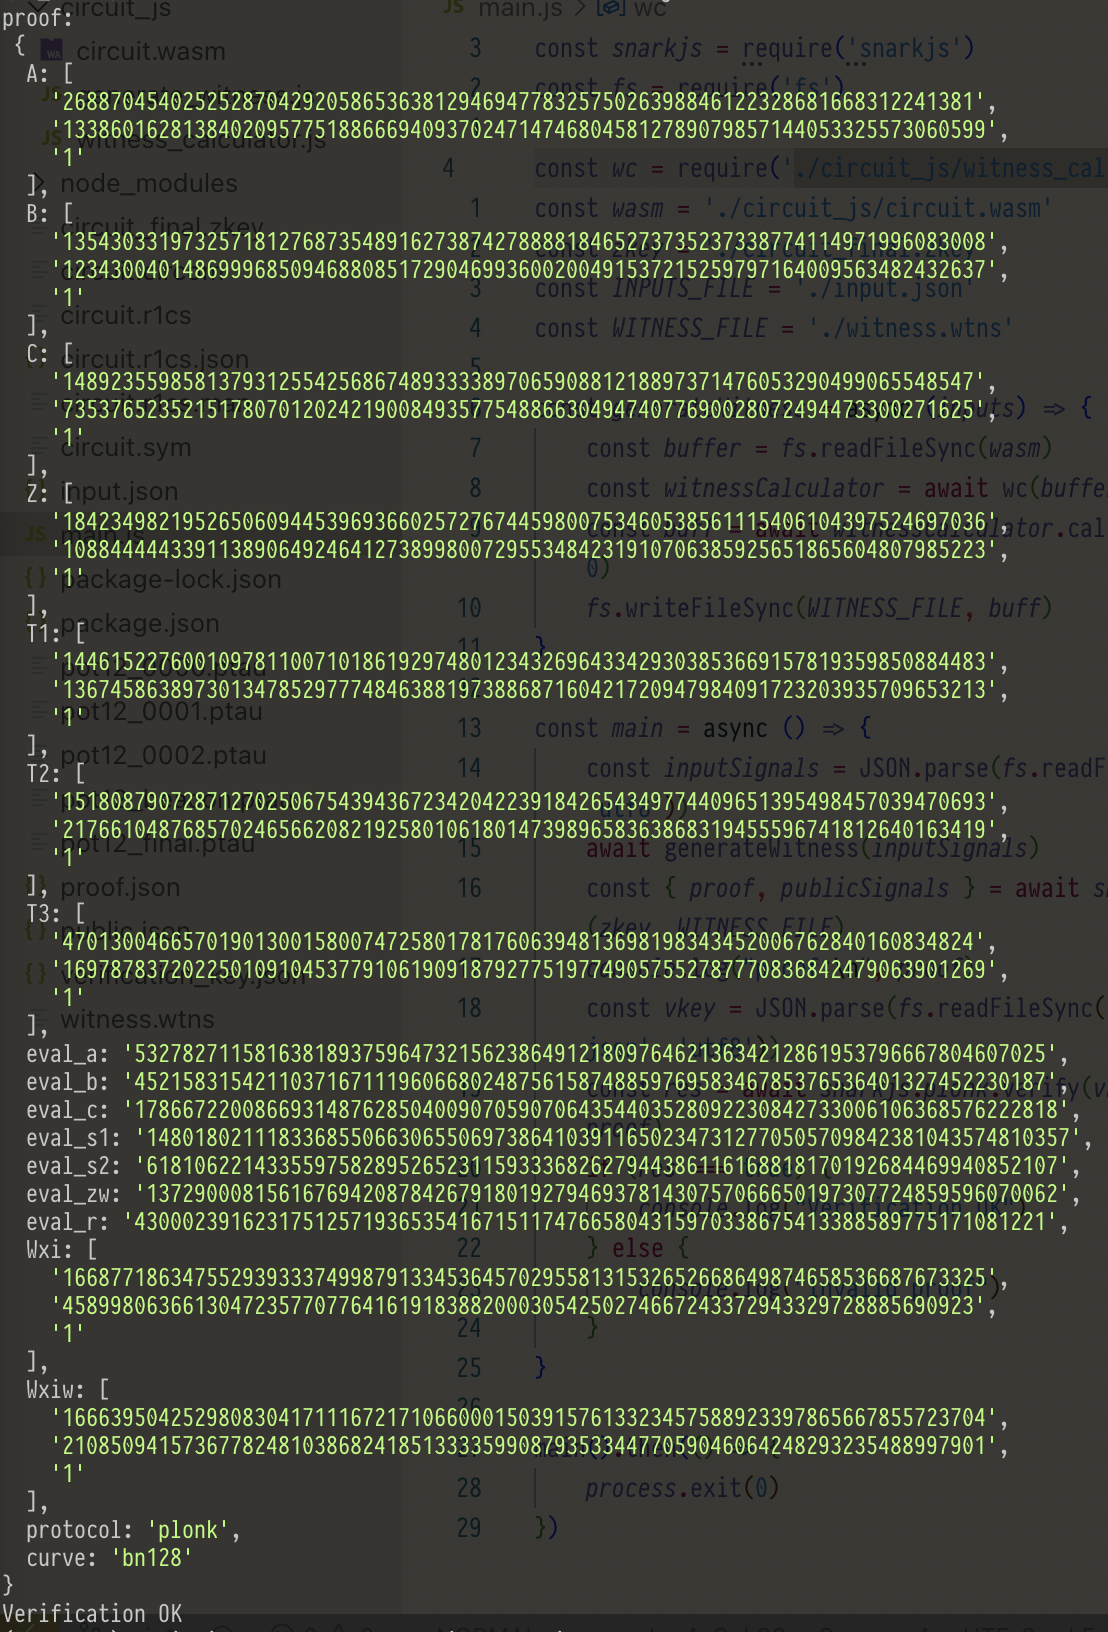
\includegraphics[width=.9\linewidth]{./img/2.png}
\caption{Screen Shot 2022-07-20 at 15.51.42.png}
\end{figure}

\item \texttt{main.js}: Commit hash \texttt{4bba17dbb299f0ac05096441554e0b8db24ab7fe} from Github repo: \url{https://github.com/tlkahn/zkworkshop-w2-a3}
\end{enumerate}
\end{document}